\documentclass[tikz,border=5pt]{standalone}
\usepackage[utf8]{inputenc}
\usepackage{tikz}
\usetikzlibrary{shapes.geometric, arrows.meta, positioning, shadows.blur, calc, fit, backgrounds}

% --- Professional Colors ---
\definecolor{processBlue}{RGB}{64, 112, 175}    % Mechanics/Synthesis
\definecolor{errorRed}{RGB}{214, 69, 65}        % Errors/Failures
\definecolor{outcomePurple}{RGB}{142, 68, 173}  % Final Mismatches
\definecolor{inputGreen}{RGB}{39, 174, 96}      % Data Source

% --- Define Styles Globally (Prevents "Paragraph ended" errors) ---
\tikzset{
    % Base style for all blocks
    process/.style={
        rectangle, 
        rounded corners=2mm, 
        minimum width=3.8cm,      
        minimum height=1.0cm,     
        text centered, 
        text width=3.5cm,         
        font=\sffamily\footnotesize, 
        draw=gray!40,
        thick,
        blur shadow={shadow blur steps=3}
    },
    % Specific styles
    sourceStage/.style={process, fill=inputGreen!10, draw=inputGreen!80!black},
    processFail/.style={process, fill=errorRed!10, draw=errorRed!80!black},
    synthesisStage/.style={process, fill=processBlue!10, draw=processBlue!80!black},
    outcomeStage/.style={process, fill=outcomePurple!10, draw=outcomePurple!80!black},
    % Arrow and Label styles
    arrow/.style={-{Stealth}, thick, draw=gray!60, rounded corners},
    groupLabel/.style={font=\bfseries\sffamily\tiny, color=gray!70, anchor=north west}
}

\begin{document}

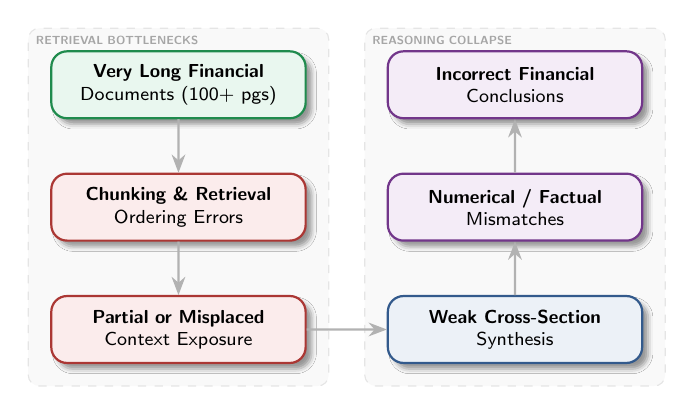
\begin{tikzpicture}[
    transform shape, 
    scale=0.85, 
    node distance=0.8cm and 1.2cm
]

    % --- LEFT COLUMN (Retrieval & Context Issues) ---
    
    % 1. Input Source
    \node (step1) [sourceStage] {
        \textbf{Very Long Financial} \\ 
        Documents (100+ pgs)
    };

    % 2. Retrieval Errors
    \node (step2) [processFail, below=of step1] {
        \textbf{Chunking \& Retrieval} \\ 
        Ordering Errors
    };

    % 3. Context Exposure
    \node (step3) [processFail, below=of step2] {
        \textbf{Partial or Misplaced} \\ 
        Context Exposure
    };

    % --- RIGHT COLUMN (Synthesis & Conclusion Failures) ---
    
    % 4. Synthesis (Bridge to the right)
    \node (step4) [synthesisStage, right=of step3] {
        \textbf{Weak Cross-Section} \\ 
        Synthesis
    };

    % 5. Mismatches (Moving Up)
    \node (step5) [outcomeStage, above=of step4] {
        \textbf{Numerical / Factual} \\ 
        Mismatches
    };

    % 6. Final Conclusion (Top Right)
    \node (step6) [outcomeStage, above=of step5] {
        \textbf{Incorrect Financial} \\ 
        Conclusions
    };

    % --- Arrows (U-Shape Flow) ---
    \draw [arrow] (step1) -- (step2);
    \draw [arrow] (step2) -- (step3);
    \draw [arrow] (step3) -- (step4); % The bridge across
    \draw [arrow] (step4) -- (step5); % Moving up
    \draw [arrow] (step5) -- (step6); % Moving up

    % --- Background Grouping ---
    \begin{scope}[on background layer]
        % Left Group: Retrieval Bottlenecks
        \node [fit=(step1)(step3), fill=gray!5, draw=gray!20, rounded corners, dashed, inner sep=8pt] (groupL) {};
        \node [groupLabel] at (groupL.north west) {RETRIEVAL BOTTLENECKS};
        
        % Right Group: Reasoning Collapse
        \node [fit=(step4)(step6), fill=gray!5, draw=gray!20, rounded corners, dashed, inner sep=8pt] (groupR) {};
        \node [groupLabel] at (groupR.north west) {REASONING COLLAPSE};
    \end{scope}

\end{tikzpicture}
\end{document}